\chapter{\label{chp:emshowers} Electron Neutrinos in Liquid Argon}

As seen in Chapter~\ref{chp:sbn}, the detection and measurement of electron neutrinos in the SBN program (and for DUNE) is essential to its success.  This chapter describes the detector signatures of electromagnetic showers, and presents a method to identify and reconstruct high energy gammas and electron neutrinos.  This work is the first observation of low energy electron neutrinos in a liquid argon time projection chamber.

Essential to detecting \nue signals is the rejection of photons from the electron candidate sample.  This chapter also presents the first demonstration of two methods to reject photons from electron candidates using data from the \argoneut detector: topological separation and calorimetric separation.

\section{Electromagnetic Showers in Liquid Argon}

An electromagnetic shower can originate in two ways. In the first, a high energy electron (produced as the outgoing lepton of a \nue interaction, for example $\nue + n \rightarrow e^− + p$) will travel through the argon freeing ionization electrons as it goes.  Eventually, the electron will scatter off of an argon nucleus. This rapid acceleration will cause the electron to emit a bremsstrahlung gamma ray. This gamma can pair produce in the presence of an Argon nucleus or orbital electron, producing a secondary high energy electron and positron. The $e^+/e^−$ pair will then each produce a cascade, similar to the original electron, until the energy is depleted: electrons or positrons emitting bremsstrahlung photons, and the photons pair producing or Compton scattering to produce more charged particles. Naturally, when all of the energy of the original particle has been exhausted by ionization of Argon from the charged particles, the shower will stop.

The second way to produce an electromagnetic shower originates with a high energy photon, also called a gamma, instead of an electron. A common source of gammas in neutrino experiments is from the decay of neutral pions: $\pi^0 \rightarrow \gamma \gamma$. When the photon interacts, it most often pair produces near a nucleus (at energies typical of those photons produced by neutrino interactions). The process is identical to the electron-induced shower after the first particles, and so electromagnetic showers from photons and electrons are only different in the original particles.

The primary method of discrimination between electrons and gammas exploits the value of the radiation length ($X_0 = 14$ cm) in argon, which is large compared to the excellent spatial resolution of TPCs. This means that a gamma can leave a visible gap between its origin and the place in the TPC where it interacts.  For an electron originating from a CC $\nu_e$ interaction no such gap will be present.

High energy gammas can, in some cases, interact at a sufficiently short distance from the neutrino's interaction vertex such that the gap between the vertex is not visible.  Further, the hadronic activity at the vertex could be invisible in the TPC data, either because it consists of only neutral particles or because the particles are below detection threshold.  Without the presence of hadronic activity to distinguish the neutrino interaction vertex, there is no possibility to observe a gap.  In this case, a second method of electron/gamma discrimination uses calorimetry at the start of the electromagnetic (EM) shower.  An electron produces ionization consistent with a single ionizing particle, whereas a gamma, at typical neutrino beam energies, converts primarily through pair production - see Figure~\ref{fig:gamma_xsec}.  The electron/positron pair produced by a gamma conversion produces ionization consistent with two single ionizing particles.  This method is only useful for the first few centimeters of the cascade - once the electromagnetic cascade develops, the amount of ionization can no longer be used to distinguish electron- and photon-induced electromagnetic showers.

% Electron-induced and photon-induced showers have a distinguishing feature in that an electron shower has only one ionizing particle at the start of the shower. Photon-induced showers instead typically have two particles - an electron and positron. Because electrons and positrons are both minimally ionizing particles, the energy deposited in the first few centimeters of a photon induced shower will be approximately double that of an electron induced shower.  

\begin{figure}[ht!]
  \centering
  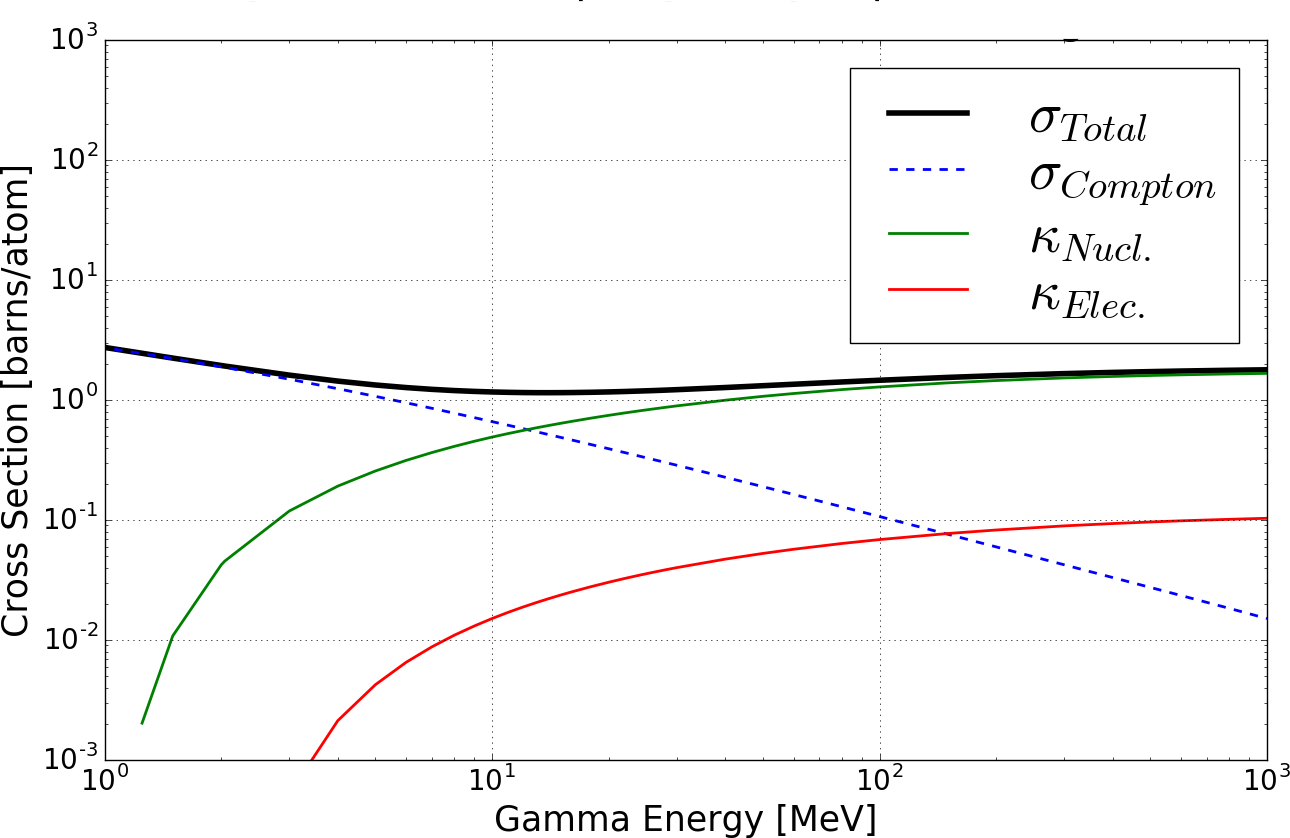
\includegraphics[width=0.65\textwidth]{emshower_figures/photonCrossSection_trimmed.png}
  \caption[Photon Cross Section on Argon]{\label{fig:gamma_xsec} The relative cross sections of high energy gammas on Argon between 1 MeV and 1 GeV. Compton and pair production cross sections are balanced at just above 10 MeV.  Data are obtained from the Xcom database \cite{Xcom}.}
\end{figure}

For the energies typical of the gammas used in this analysis the distribution of gamma conversion distances is shown in Figure \ref{fig:photon_conversion_dist}.  There are gammas that convert very close to the generation point (here, 7\% of the gammas convert within a centimeter).  The definition of ``too close'' depends on the analysis being performed, however, there will always be a fraction of gammas for which a topological based cut is insufficient to tag them as gammas.  In the ArgoNeuT detector, the minimal resolution of a gamma gap is approximately one wire spacing (4~mm). In neutrino interactions with hadronic activity at the vertex, it is possible that other particles can obscure the start of an electromagnetic shower.  In this case, even gaps as large as a few centimeters can become unidentifiable.

\begin{figure}[h!]
  \centering
  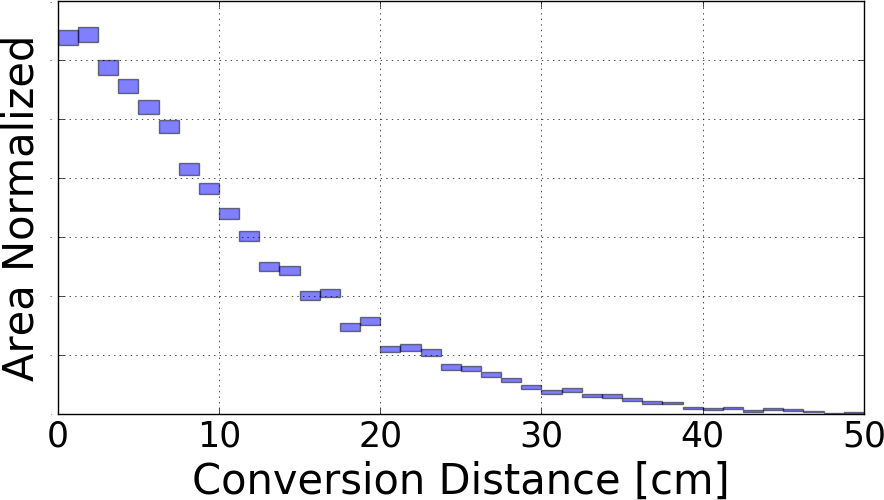
\includegraphics[width=0.75\textwidth]{emshower_figures/photon_conversion_dist_trimmed.png}
  \caption[Photon Conversion Distance]{The conversion distance of each gamma in the Monte Carlo sample used for this analysis, which is about 7000 gammas in the energy range of several hundred MeV, as modeled by GEANT4 \cite{Agostinelli:2002hh}.}
  \label{fig:photon_conversion_dist}
\end{figure}

The calorimetric separation of electrons and photons, using the amount of ionization measured at the start of the shower, depends on the photon interacting through pair production and not Compton scattering.  As seen in Figure~\ref{fig:gamma_xsec}, the scatter cross section of photons is dominated by pair production above 100 GeV, though the Compton cross section remains relevant up to 1 GeV of photon energy.  Figure~\ref{fig:relative_gamma_xsec} shows the relative probability that a photon will interact through either Compton or pair production channels.  Importantly, a photon that interacts through Compton scatter can not be distinguished via calorimetry from an electron.  Instead, only a topological separation can be used on an event-by-event basis for Compton-scatter photons.  In most neutrino experiments such as the SBN program \cite{Antonello:2015lea} and DUNE \cite{DUNE}, the high amounts of photons produced compared to expected electron neutrino events makes the fraction of Compton scatter photons a relevant background.  Therefore, both methods of separation are crucial.

\begin{figure}[ht!]
  \centering
  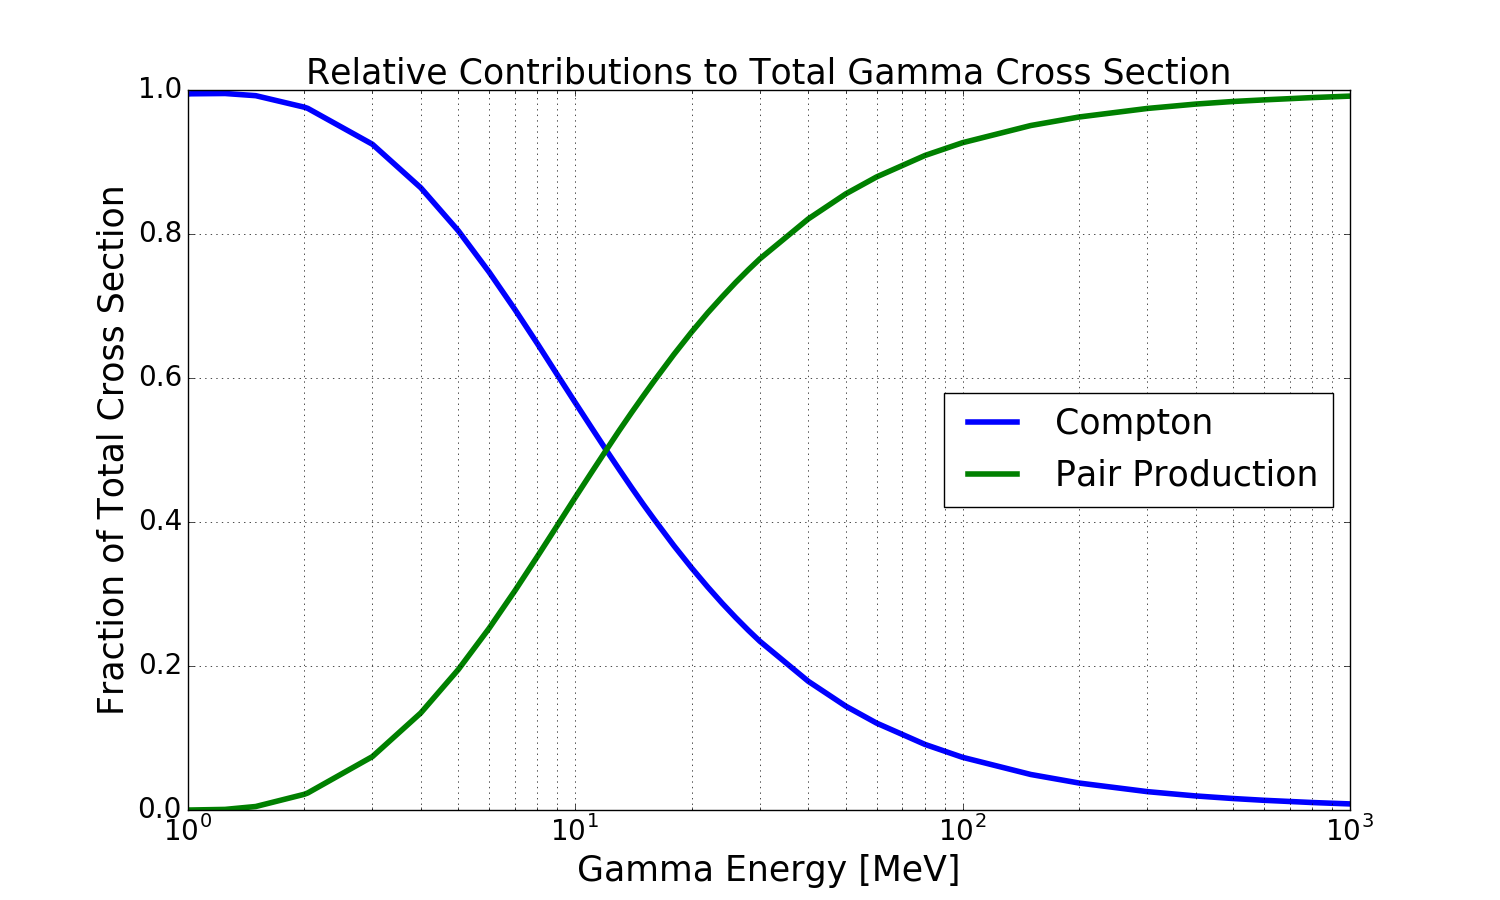
\includegraphics[width=0.65\textwidth]{emshower_figures/relative_photonCrossSection.png}
  \caption[Comparison of Compton to Pair Production Cross Section]{\label{fig:relative_gamma_xsec} The cross section of high energy gammas on Argon between 1 MeV and 1 GeV.  Here, $\kappa$ refers to the pair production cross section for the nuclear field and electron field.  Compton and pair production cross sections are balanced at just above 10 MeV.  Data are obtained from the Xcom database \cite{Xcom}.}
\end{figure}


\subsection{Selection of Electromagnetic Showers in \argoneut}

To validate the separation of electromagnetic showers in \lartpcs, a study was performed using the neutrino events from the \argoneut detector to select samples of electron candidate and photon candidate events.  A sub-sample of the \argoneut data set containing electromagnetic showers is isolated first, and this sub-sample is used to select well defined electron and gamma events by visual scanning.


\begin{figure}[htb]
\centering
\includegraphics[height=2.in]{emshower_figures/princcomp_area_proper.pdf}
\includegraphics[height=2.in]{emshower_figures/modhitdensarea_proper.pdf}
\caption[Discrimination variables for Shower Identification]{\label{fig:separation} Principal Component Eigenvalue (top) and ``Modified hit density'' (bottom) calculated for single electron showers(red) and muon tracks (blue).}
\end{figure}

Selecting the sub-sample of electromagnetic showers is based on information from the 2-dimensional clusters of charge depositions (hits) in each wire plane. First, empty events and events with only track like particles are removed from the sample using an automated filter. This filter considers two-dimensional clusters of hits made with the LArSoft package \cite{Church:2013hea}, and calculates several parameters of these clusters to differentiate between track-like and shower-like clusters. 

The two most successful metrics in separating tracks and showers for well clustered events are the principal eigenvalue of a principal component analysis (PCA), and a direction corrected hit density of the cluster:
\begin{itemize}
  \item {\bf Principal Component Eigenvalue:} A principal component analysis (PCA) \cite{PCA} takes a collection of N dimensional points and numerically finds the orthonormal coordinate system that best aligns to the data.  The goodness-of-fit metrics in the PCA analysis are the eigenvalues of the transformation matrix between the initial coordinate system and the best fit.  In this analysis, we use the 2D reconstructed charge depositions (hits) in the wire-time views of the collection plane TPC data and perform a principal component analysis on each cluster.  For track like particles, which have strong directionality, the first eigenvalue of the analysis is quite high, close to 1.  For shower like clusters, the direction of the shower and it's transverse direction are less obviously separated, and the principal eigenvalue is lower than 1.  
  \item{\bf Direction Corrected Hit Density:}  A showering event is defined significant activity in the TPC that is resolved away from the primary axis of the particle.  That is, a shower has many hits reconstructed as it travels through the TPC, whereas a track generally has one charge deposition detected per step through the TPC.  Measuring the hit density, defined as hits per unit distance, along a particle can thus discriminate between tracks and showers.  Since hits are only reconstructed on wires, and tracks and showers need not be perpendicular to the wires, the hit density is corrected to account for the fact that high angle tracks and showers (more parallel to the wires) have relatively fewer hits reconstructed.
 \end{itemize}


For this analysis, a cut is made on the value of $log(1-E.V._{PCA}) > -5$ as seen in Figure~\ref{fig:separation}.  $E.V._{PCA}$ is the first eigenvalue of the PCA analysis.  This corresponds to rejecting all clusters that have a principal eigenvalue greater than $\sim$0.999.  Events with a corrected hit density greater than 1.5 hits per cm are kept.  Figure~\ref{fig:separation} shows these separation parameters obtained using Monte Carlo simulations of single electrons as a model for electromagnetic showers, and single muons and protons as an archetype for tracks. 

An additional requirement is that a shower-like cluster in on plane should correspond to an analogous cluster in the second plane at the same drift time. This removes spurious events tagged as showers due to wire noise or other sources in just one plane.

Finally, an additional set of criteria is applied using all of the hits in a single view in an event as a single cluster. These criteria remove high-multiplicity $\nu_{\mu}$ deep inelastic scatter events and cosmic ray events which resulted in a large amount of total charge in an event. 

This procedure resulted in sample of ArgoNeuT events that contained mostly EM-shower events, from which the final electron and gamma samples are selected.

When a gamma is produced in an interaction in argon, it will travel some distance, typically less than 50~cm in argon (for a 500 MeV gamma), before it interacts with the argon and induces an electromagnetic shower.  Thus there is often a gap between the origin of the gamma and the start of the electromagnetic shower. Unless there is other activity in the detector at the location of gamma production, the gap is impossible to detect.  Therefore, two types of events are classified as gamma candidates, based on the observation of charged protons or pions at a neutrino interaction vertex: electromagnetic showers pointing back to charged particle activity at a vertex with hadronic interaction, and Neutral Current $\pi^0$ events where two electromagnetic showers project back to a common point.  In the second case, hadronic activity at the vertex is allowable but not required.  Examples of both types of gamma interactions are shown in Figure~\ref{fig:photons}.  Gammas that are unable to be positively identified purely through topological considerations - if, for example, the electromagnetic shower is the only activity in the detector - are not used in this analysis.



\begin{figure}[ht]
\centering
\includegraphics[width=\textwidth]{emshower_figures/PhotonEvents.pdf}
\caption[Photon Events in \argoneut]{\label{fig:photons} Examples of gamma candidate events.  The top row are the induction views and the bottom row are the collection views of two events. In both cases, the key identifying feature is the gap between the showers and the other activity to which they point backwards.  In the (bottom) collection planes, there is a block of 5 wires that are inactive.}
\end{figure}

For a sample of electrons, this analysis targeted electron neutrino events as the electron shower candidates.  To maximize purity, an electromagnetic shower is selected as an electron candidate only in events that also exhibited hadronic activity at the vertex {\em without} the presence of a gap between the shower and other particles.  In addition, events with a track like particle matched to a muon in the MINOS near detector are rejected.  This ensures that the contamination from $\nu_\mu$ charged current events with high bremsstrahlung activity is negligible.  Examples of electron candidates are shown in Figure~\ref{fig:electrons}. In total, 37 electron candidate showers and 274 gamma candidate showers are selected for this analysis.



\begin{figure}[ht]
\centering
\includegraphics[width=\textwidth]{emshower_figures/ElectronEvents.pdf}
\caption[Electron Candidate Events in \argoneut]{\label{fig:electrons} Examples of $\nu_e \rightarrow e$~CC events.  The top row are the induction views and the bottom row are the collection views of two events. In both cases, there is no observable gap between the shower and the hadronic activity.In the (bottom) collection planes, there is a block of 5 wires that are inactive due to a bad electronics connection in the detector.}
\end{figure}


\section{Reconstructing Electromagnetic Showers in \lartpcs}

To reconstruct electromagnetic showers in \lartpcs, a procedure described in Section~\ref{sec:shower_reconstruction} is applied.  In general, the raw data from the detector must be deconvolved to mitigate noise sources, and a peak finding algorithm is applied to the signal from each wire to find charge depositions, known as hits. The integral of the ADC count in each hit is used to calculate the charge $dQ$ using an (ADC$\times$Timetick)/Coulomb conversion constant.  The constants are obtained using the procedure described in \ref{subsec:lartpc_calibration}, which follows the procedure in \cite{Anderson:2012mra}.

The most difficult step in the reconstruction of electromagnetic showers, by far, is deciding which hits in an interaction are associated with the shower. For the events selected to demonstrate electron/gamma separation, the hits were assembled into appropriate clusters manually.

In order to measure dE/dx correctly, it is extremely important to precisely determine the start point and direction of the shower. In particular, the start point and direction are needed to measure the {\em first} several centimeters of the shower before the development of the electromagnetic cascade. Once the shower develops, the electron and gamma populations become significantly less distinguishable (see Section \ref{sec:dedx_calcs}). 


\subsection{Reconstruction Algorithms}
\label{sec:shower_reconstruction}

\begin{figure}[h!]
  \centering
  \includegraphics[width=\textwidth]{emshower_figures/iterative_start_point.pdf}
  \caption[Diagram of the 3D start point algorithm.]{Diagram of the 3D start point algorithm.}
  \label{fig:iterative_start_point}
\end{figure}

The 3D start point is initially calculated from the intersection point of the wires where the two 2D start points are found and their position in the drift time coordinate.  The start point in 3D is improved using an iterative algorithm, and illustrated in Figure \ref{fig:iterative_start_point}.

An initial guess, the point in black, is made for the start point based on the 2D start points (yellow stars in each plane).  The start point in 3D is projected into each plane, and the error in the 3D start point is the sum (over each plane) of the distance between the true start point in each plane and the projection of the 3D point.  Six additional points, along the detector coordinates (in the $\pm$ x, y, and z directions), are also projected into each plane, and the error of each point is computed similarly (black dashed lines show the distance between projection and true start point).  The point with the smallest summed error is chosen as the better 3D start point, and the algorithm makes an additional six guesses around it.  If the central point (in black) is chosen as the best fit point, the distance the other 6 points are offset from it is decreased and the algorithm repeats.  This procedure is repeated until the algorithm can no longer improve the accuracy of the 3D start point.  The initial offset from the central point for the 6 auxiliary points is 5 centimeters, and it decreases by 2\% for each successful iteration.  As seen in Figure~\ref{fig:shower_reco}, the 3D start point resolution is generally better than 1 cm.

\begin{figure}[h!]
  \centering
  \includegraphics[width=\textwidth]{emshower_figures/iterative_start_dir.pdf}
  \caption[Diagram of the 3D start direction algorithm.]{Diagram of the 3D start direction algorithm.}
  \label{fig:iterative_start_dir}
\end{figure}


Similar to the 3D start point, the 3D axis is computed using an iterative projection matching algorithm.  The standard TPC trigonometric formula is used to compute an approximate 3D axis based on the angle of each shower in the collection and induction plane:

\begin{align}
  \theta &= \text{arccos}\frac{m}{\sqrt{l^2 + m^2 + n^2}}, \\
  \phi &= \text{arctan}\left(\frac{n}{l}\right) 
\end{align}
where
\begin{align}
l &= sign(t_{end} - t_{start}), \\
m &= \frac{1}{2 \text{sin}(\alpha)}\left(\frac{1}{\Omega_0} - \frac{1}{\Omega_1}\right), \\
n &= \frac{1}{2 \text{cos}(\alpha)}\left(\frac{1}{\Omega_0} + \frac{1}{\Omega_1}\right).
\end{align}

Here, $\theta$ represents the polar angle in 3D with respect to the z axis (approximately the beam direction).  $\phi$ is the azimuthal angle in the x-z plane, with $\phi$ = 0 along the z axis, and  $\alpha$ is the angle of the wire planes with respect to the vertical direction, which in ArgoNeuT is 60 degrees.  $\Omega_0$ and $\Omega_1$ are the tangents of the 2D angles of the shower measured in each plane.  $t_{start}$ and $t_{end}$ are the start and end points of the cluster, such that $l$ is positive if the shower points away from the wires and positive the shower points towards the wires.

\begin{figure}[htbp]
   \centering
   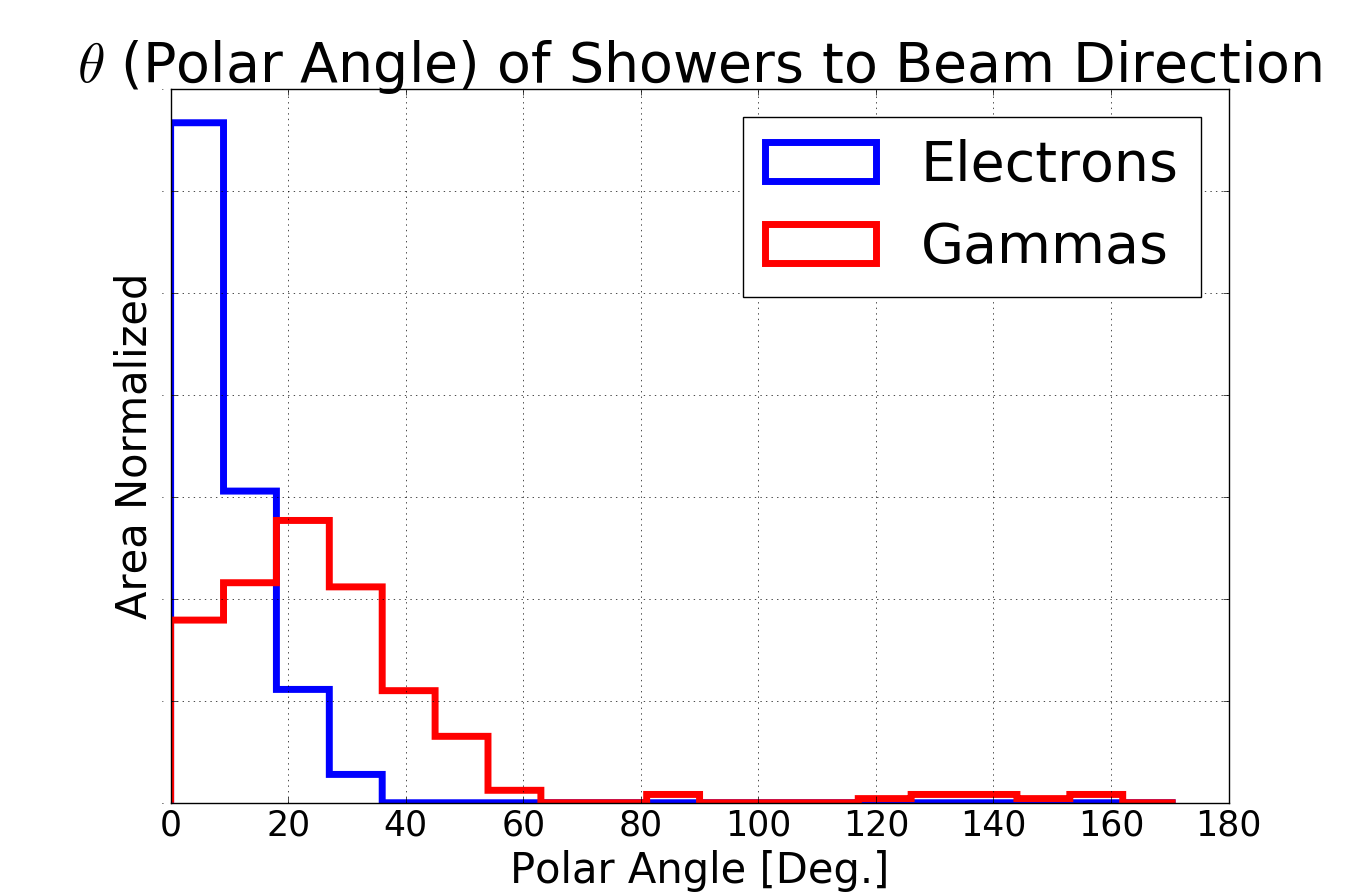
\includegraphics[height=2in]{emshower_figures/theta_distribution.png}
   \caption[Angular Distributions of Electromagnetic Showers.]{The distribution of the polar angle of events with respect to the Z direction (approximately the beam direction).  The electron sample is very forward going, and the gamma sample has a wider distribution of angles. }
   \label{fig:geomety_dists}
 \end{figure} 

\begin{figure}[htbp]
   
   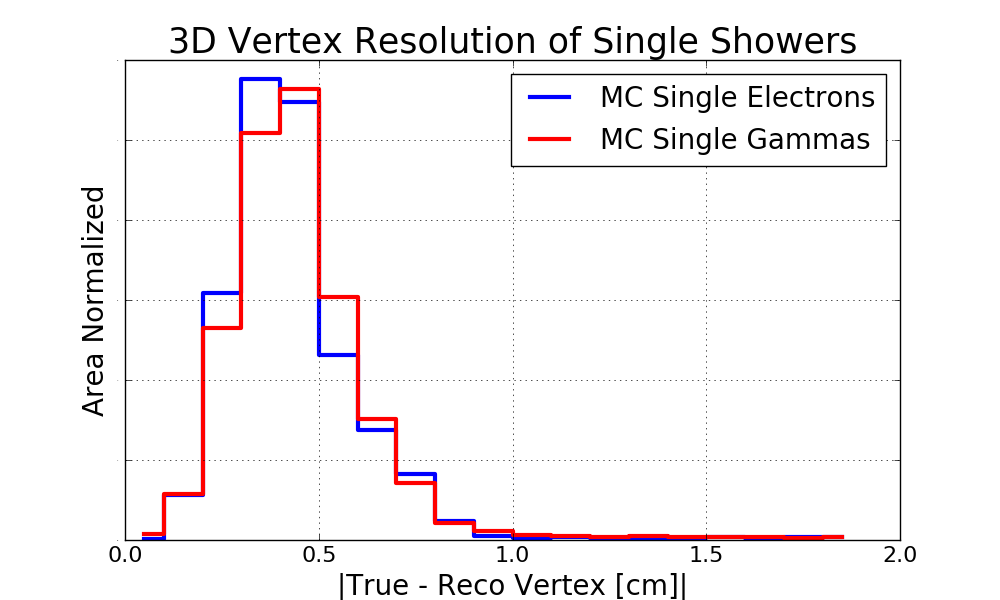
\includegraphics[width=0.45\textwidth]{emshower_figures/3d_resolution.png}
   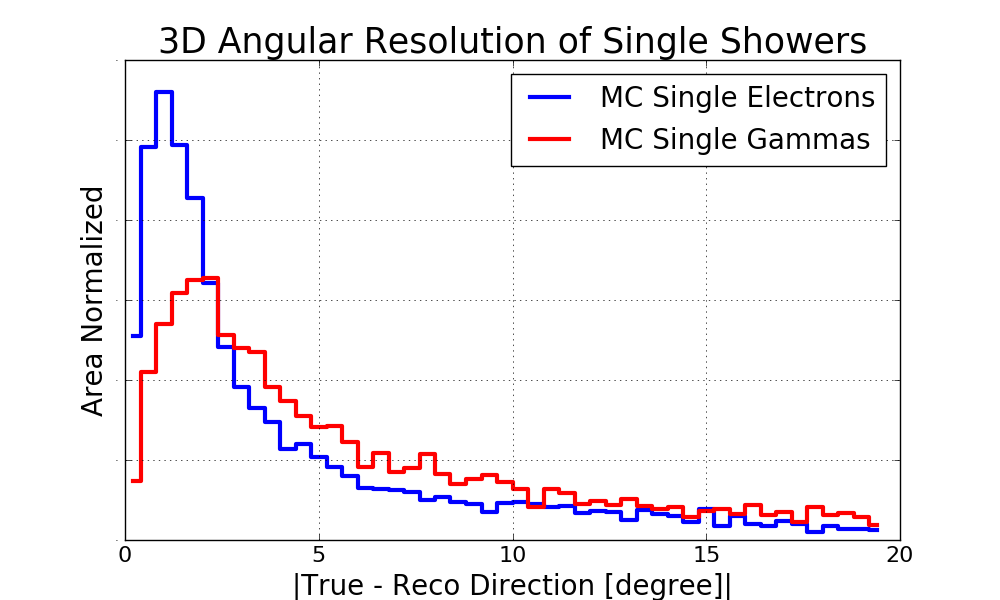
\includegraphics[width=0.45\textwidth]{emshower_figures/AngularResolution.png}
   \caption[Resolution of Electromagnetic Showers]{The calculated resolution of the 3D start point (left) and angular resolution (right) for single electromagnetic showers generated with the LArSoft package.  The angular resolution for gammas is slightly worse than for electrons because the gamma sample is at lower energy, and hence has fewer depositions (hits) in the TPC.}
   \label{fig:shower_reco}
 \end{figure} 


The reconstructed 3D axis is then projected into each plane, and the slope (in 2D) is compared against the slope of the electromagnetic showers in each plane.  Based upon the quality of the match between the projection and the 2D slopes, the 3D axis is adjusted until the best fit is obtained - see Figure~\ref{fig:iterative_start_dir}.  An initial guess, the arrow in black, is made for the start direction based on the 2D start directions (red arrows in each plane).  The start direction in 3D is projected into each plane, and the error in the 3D start direction is calculated.  An additional set of 3D directions (gray arrows) are also projected into each plane.  If the central direction (in black) is chosen as the best fit direction, the angular separation between it and the other (gray) directions is decreased and the algorithm repeats.  This procedure is repeated until the algorithm can no longer improve the accuracy of the 3D start direction.

The angular resolution for electromagnetic showers, shown in Figure~\ref{fig:shower_reco}, is generally quite good (better than 5 degrees) though there is a substantial tail.  However, for this analysis, the poor resolution in a few measurements of the 3D axis has a minimal effect on the dE/dx calculation.  This is due to the fact that the majority of the events are forward going, as shown in Figure \ref{fig:geomety_dists}.  Therefore a moderate uncertainty in the 3D angle leads to only a small uncertainty in the effective wire pitch, described below, and a small uncertainty in dE/dx.

\begin{figure}[htb]
   \centering
   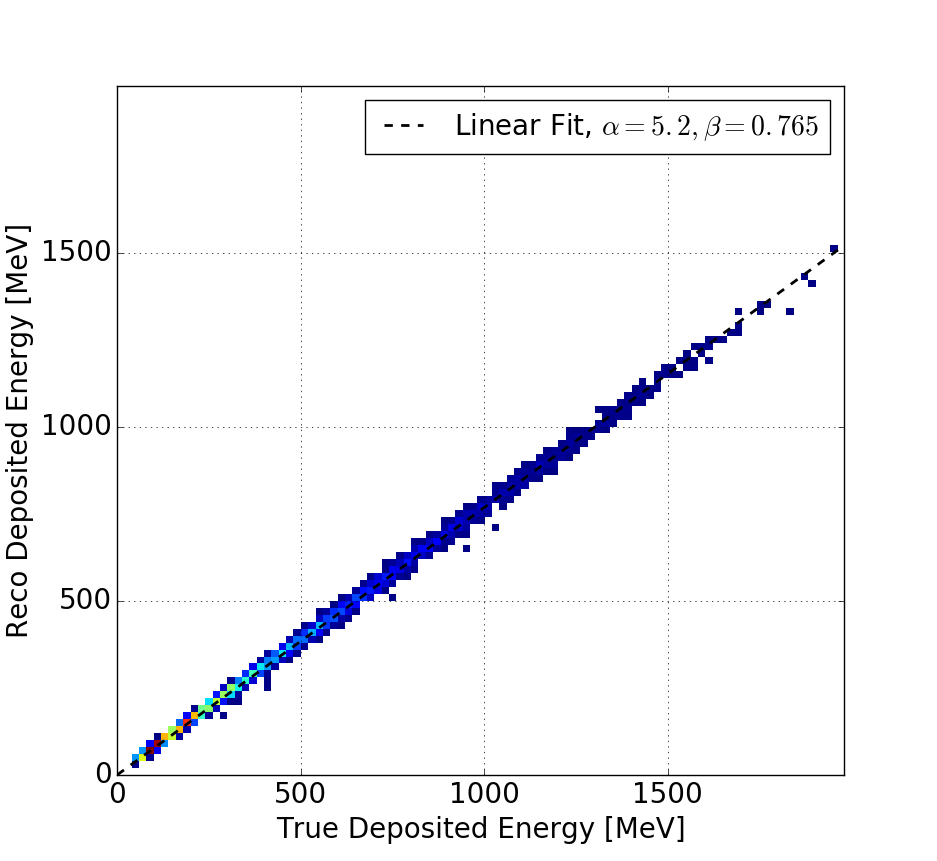
\includegraphics[width=0.9\textwidth]{emshower_figures/depositedEnergyCalibration.png}
   \caption[Deposited Electron Energy]{The reconstructed, deposited energy of an electron shower compared to the true, simulated deposited energy.}
   \label{fig:depositedE}
 \end{figure} 

Since an electromagnetic shower is a combination of many single ionizing particles - electrons and positrons - and is not composed of highly ionizing stopping particles - i.e., protons - the measured charge on the sense wires in the peak of the showering activity is a sum of many minimally ionizing particles.  Therefore, to calculate the total energy deposited by an electromagnetic shower, each deposition collected is corrected by a recombination amount that is proportional to a minimally ionizing particle.  All of the energy depositions, once corrected, are summed into a final measure of the reconstructed, deposited energy.  Figure~\ref{fig:depositedE} shows the relationship between the true deposited energy from the simulation and the reconstructed deposited energy of electron showers.  The correlation between the two is quite strong, though there is a significant and consistent deficit of reconstructed energy compared to the true energy.  This deficit arises from the very small ionizations coming from very low energy photons in the argon, which are far from the main shower and either below detection threshold or not spatially associated with the electromagnetic shower.

Lastly, for the calorimetric separation of electrons and gamma to succeed, the dE/dx metric must be well reconstructed. As the charge depositions are measured discretely in 2D on single wires, in each of the wire planes we use the 3D axis of the shower to calculate an ``effective'' wire pitch between hits.  This effective pitch is, in other words, the real distance in the TPC that a particle travels between its two projections (hits) on adjacent wires. Figure \ref{fig:effective_pitch} shows the distributions of effective pitches for the electron and gamma samples.  The effective pitch is at least the wire spacing, which is 0.4 cm in ArgoNeuT.  The gamma distribution shows a slightly higher effective pitch, which is expected from Figure \ref{fig:geomety_dists} showing that the gammas are at slightly higher angles to the wire planes than the electron sample.  In the calculation of dE/dx, the effective pitch is used as the estimate of `dx'.

\begin{figure}[htbp]
  \centering
  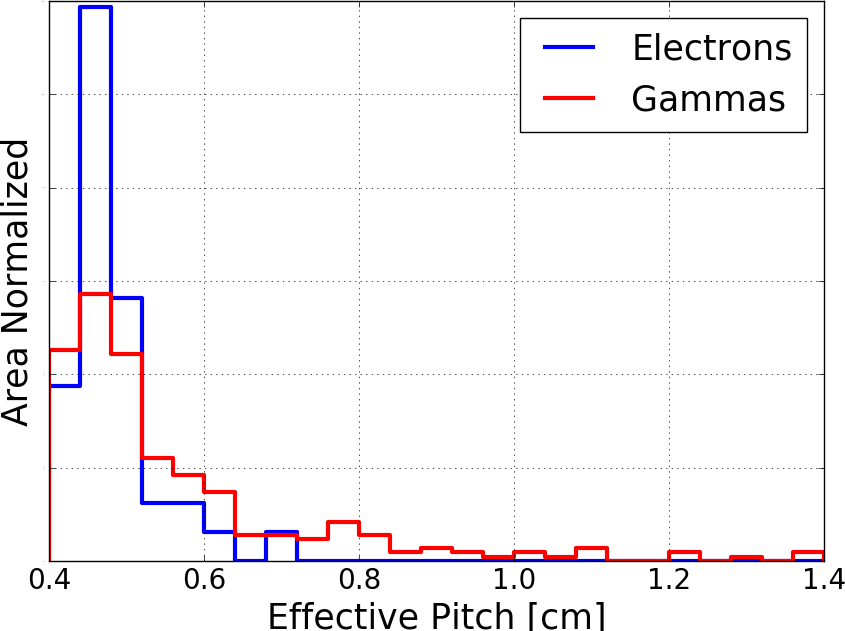
\includegraphics[width=0.5\textwidth]{emshower_figures/effective_pitch_trimmed.png}
  \caption[Effective Pitch]{The effective pitch for the electron and gamma samples used in this analysis.  The effective pitch is a measure of how far a particle travels between depositions of charge recorded on adjacent wires.  }
  \label{fig:effective_pitch}
\end{figure}

\begin{figure}[htb]
  \centering
  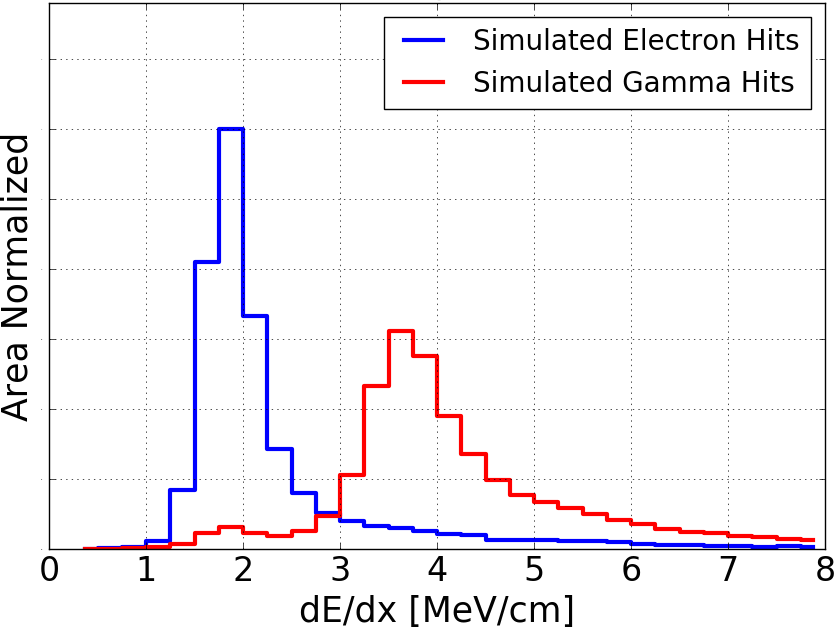
\includegraphics[width=0.75\textwidth]{emshower_figures/mcLandaus_trimmed.png}
  \caption[Simulated Single Hit Distributions for Showers]{Distribution of $dE/dx$ for all hits at the start of the shower for the electron and gamma samples using Monte Carlo.}
  \label{fig:mc_landaus}
 \end{figure} 

A valuable cross-check of this sample of events is the distribution of every $dE/dx$ deposition measured at the start of the shower, from all the events in the selected sample.  Figure~\ref{fig:mc_landaus} shows this distribution for the Monte Carlo simulation of both electrons and photons.  The electron hits follow a Gaussian-convolved Landau distribution, while the photon distribution is more complicated due to the presence of two single ionizing particles at the start of both showers.  In addition, the photon distribution includes contributions from photons that Compton scatter instead of pair producing.

\begin{figure}[htb]
  \centering
  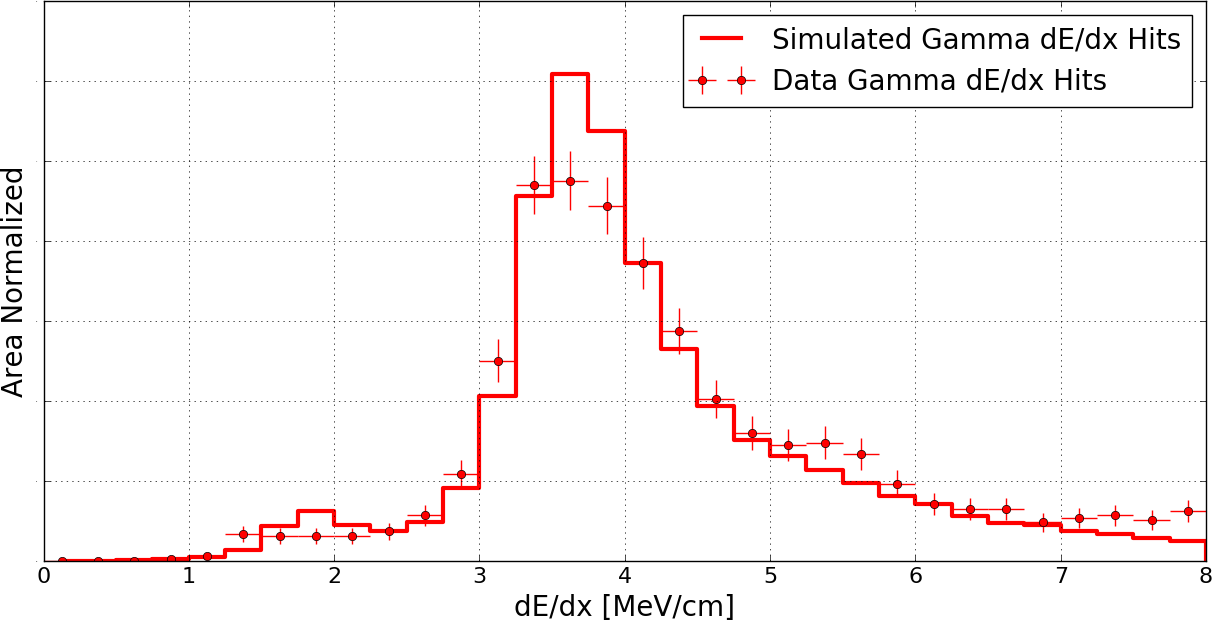
\includegraphics[width=0.99\textwidth]{emshower_figures/photons_landau_trimmed.png}
  \caption[Photon Landau Distribution]{Distribution of $dE/dx$ for all hits at the start of the shower for the gamma sample.}
  \label{fig:photon_landau}
 \end{figure} 

For the gamma sample, the comparison of data and simulation is shown in Figure~\ref{fig:photon_landau}.  Since the gamma sample is produced entirely by selecting showers with a displaced vertex, the purity of the gamma sample is 
taken to be nearly 100\% in this analysis.


For the electron sample, we can not assume that the purity of the sample is 100\% based on topology alone.  As seen in Figure~\ref{fig:photon_conversion_dist}, a non-negligible amount of gammas will convert at a sufficiently short distance that they will get selected as electrons in a topological based cut.  Hadronic activity at the vertex can also obscure the presence of a gap from a gamma.  Therefore, the distribution of electron-like $dE/dx$ hits analogous to Figure~\ref{fig:photon_landau} is expected to be modeled by a combination of electron and gamma showers in Monte Carlo.

In Figure~\ref{fig:mc_landaus}, the simulated $dE/dx$ distributions for electrons and gammas are shown.  These two distributions are used to fit to the equivalent distribution of the electron-candidate data sample, using a linear combination of electron and gamma Monte Carlo such that the normalization is fixed.  The $\chi^2$/dof is minimized between the (area normalized) data distribution and the combination of the electron and gamma distributions from Monte Carlo.  The best fit is shown on the right side of Figure~\ref{fig:electron_landau}.  The $\chi^2$/dof decreases from 2.78 with no gamma contamination to 1.02 when a gamma contamination is included at 20 $\pm$ 15\%.  This represents a direct measurement of the misidentification rate of the topological selection of electrons for this particular analysis, and demonstrates a method to measure this mis-ID rate in future electron neutrino searches in LArTPCs.

\begin{figure}[htb]
  \centering
  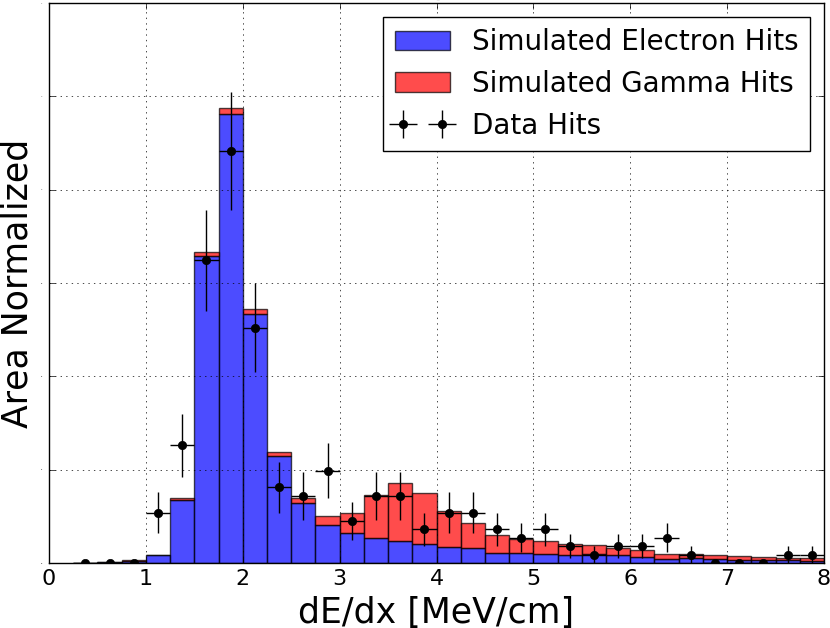
\includegraphics[width=0.85\textwidth]{emshower_figures/fitted_electron_distribution_trimmed.png}
  \caption[Electron Landau Distribution]{All $dE/dx$ hits from the electron candidate sample, compared to a sample of Monte Carlo comprised of 80\% electrons and 20\% gamma.}
  \label{fig:electron_landau}
\end{figure} 


As a final verification of the reconstruction, the measured distribution for the electron candidates is corrected by subtracting the gamma distribution from Figure \ref{fig:electron_landau}, scaled by the 20\% found above.  This background subtracted distribution is fit with a Gaussian-convolved Landau distribution to determine the most probable value of charge deposition.  In particular, the most probable value of $dE/dx$ for electron like hits is consistent with the theoretical values as shown in Figure~\ref{fig:mpv_electrons}. For electrons above 100 MeV/c, as this sample is, the theoretical expectation of the most probable ionization is 1.77 MeV/cm.  This is in good agreement with the fitted value of 1.74 MeV/cm.

\begin{figure}[htb]
  \centering
  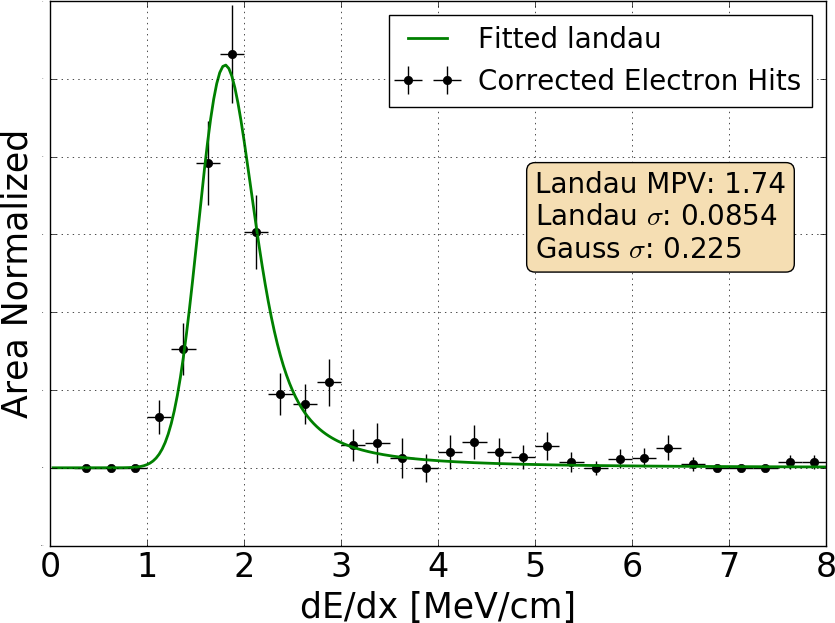
\includegraphics[width=0.85\textwidth]{emshower_figures/fitted_electron_landau_trimmed.png}
  \includegraphics[width=0.85\textwidth]{emshower_figures/mpv_electrons.pdf}
  \caption[Background Subtracted Electron Landau Distribution]{(Top) Background subtracted distribution of the hits at the start of the electron showers, with a fitted Gaussian-convolved Landau .  (Bottom) Most probable value of ionization as a function of momentum for particles traversing liquid argon.}
  \label{fig:mpv_electrons}
 \end{figure} 

\FloatBarrier

\section{\label{sec:electrons} Detection of Electron Neutrinos}

To verify that the sample of electron-candidate events are predominantly electron neutrino events, the kinematic behavior of the electron-candidate sample has been studied.  Due to the small active volume of the ArgoNeuT detector, the electromagnetic showers are poorly contained and the reconstructed electron energy is not a measurable quantity.  Instead, we measure the distribution of reconstructed {\em deposited} energy, compared to a simulation of electron neutrino events using the electron neutrino and anti-neutrino flux shown in Figure~\ref{fig:argoneut_flux}.  This flux used to simulate the electron neutrino events is generated with a simulation of the NuMI beam with FLUKA \cite{Aliaga:2016oaz}.  The mean energy of the electron anti-neutrinos is 4.3 GeV, while the mean energy of electron neutrinos is 10.5 GeV.  As seen, the beam is predominately electron anti-neutrinos.

Figure~\ref{fig:electron_kinematics} shows the kinematic distribution of the electron events' deposited energy and angle $\theta$.  For both the deposited energy and the polar angle $\theta$, the agreement between data and Monte Carlo is good.  For the measurement of deposited energy, the Monte Carlo deposited energy is scaled by 24.5\% to model the reconstruction inefficiencies as observed above.

In Figure~\ref{fig:electron_kinematics}, both the deposited energy and reconstructed angle are area normalized independently for both data and simulation.  Due to the fact that the electron candidate events were selected manually from a sample of showering events, we are unable to accurately estimate the efficiency of electron neutrino selection.  Therefore, an absolute comparison of data and Monte Carlo is not possible, and not presented here.  For the same reason, the measurement of the electron neutrino scatter cross section is also not presented.

Regardless, this analysis is the first observation of low energy electron neutrinos in a liquid argon time projection chamber.  This is an essential step towards the successful analyses of \uboone, the SBN Program, and DUNE.


\begin{figure}[htbp]
  \centering
  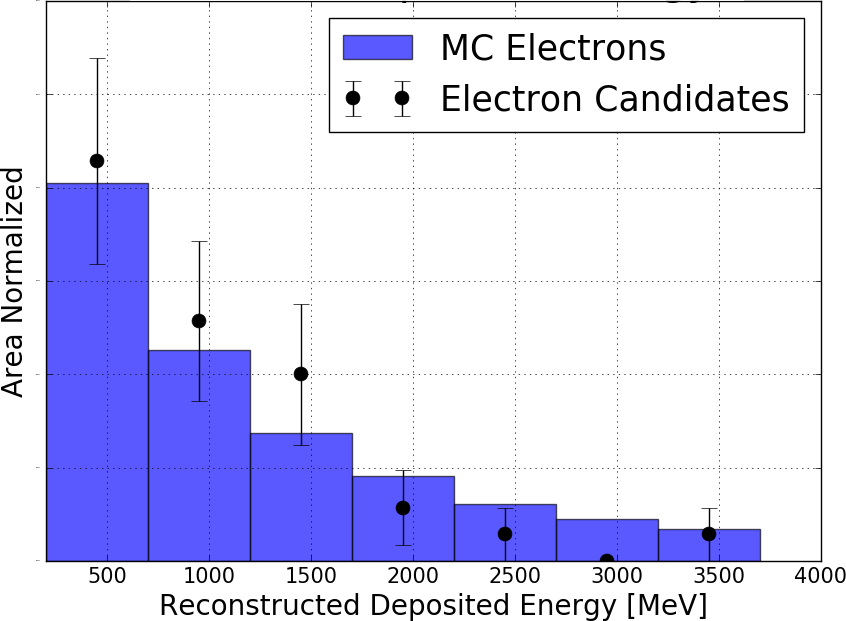
\includegraphics[width=0.48\textwidth]{emshower_figures/depE_corrected_trimmed.png}
  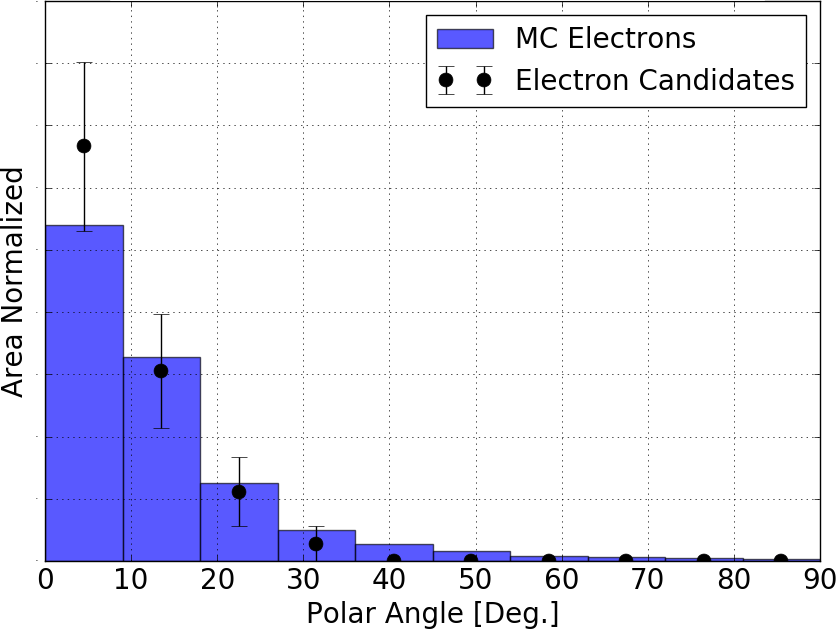
\includegraphics[width=0.48\textwidth]{emshower_figures/angle_comparison_trimmed.png}
  \caption[Electron Kinematic Variables]{(Left) Electron deposited energy. (Right) Electron polar angle.  In general, these kinematic variables agree with the simulation, despite low data statistics.msd2}
  \label{fig:electron_kinematics}
\end{figure}

\section{\label{sec:dedx_sep} $dE/dx$ Separation}


Once an electromagnetic shower has been identified and reconstructed, the information from the charge depositions at the start of the shower needs to be aggregated into a single dE/dx metric. 

In the previous section, the conversion from $dQ/dx$ (the measured charge per unit centimeter), to $dE/dx$ (deposited energy per unit centimeter) is computed using a nonlinear model of the recombination of electrons and argon ions \cite{Birks, Acciarri:2013met}.  In considering the ionization at the start of a gamma induced shower where an electron and positron pair are present, we assume the ionization clouds of the two particles are sufficiently separated such that a non linear model incorrectly inflates the $dE/dx$ from a $dQ/dx$, for higher values of $dQ/dx$.  Thus, the $dE/dx$ separation is computed using a minimally ionizing particle scale recombination correction for all charge depositions at the beginning of the shower in the electron and gamma samples.  While this is not applicable for highly ionizing fluctuations, it prevents an over estimation of the $dE/dx$ of gammas which artificially inflates the calorimetric separation power. 

For a given event there is not a statistically large sample of energy depositions to use for measuring a robust average $dE/dx$.  Given the Landau nature of the energy deposition fluctuations away from the most probable value, it is not surprising that an aggregate metric will tend towards higher energy depositions per centimeter than the most probable value.   For this analysis, when computing the $dE/dx$ separation metric for a shower all of the hits within a rectangle of 4 cm along the direction of the shower and 1 cm perpendicular to the shower are collected, and the median is computed.

\section{\label{sec:dedx_calcs} $dE/dx$ Calculation Methods}

While investigating the methods to convert a sample of hits (per shower) into a single variable, three promising $dE/dx$ metrics were developed:
\begin{enumerate}
  \item {\bf Outlier Removed Mean}: For every hit considered for each shower (within a certain distance from the start), the mean $dE/dx$ of the hits is calculated, as well as the RMS.  The hits that are outside of the mean $\pm$ the RMS are then rejected, and the mean of the remaining hits is recomputed and used.
  \item {\bf Median}: The same initial set of hits as above is used.  However instead of rejecting outliers a median is calculated.  In particular, this method is robust against single high or low fluctuations.
  \item {\bf Lowest Moving Average}: For the same set of N initial hits, a moving 3 hit average is calculated.  For example, for N hits, the average is calculated of the hits (1,2,3), then the hits (2,3,4), etc. until the hits (N-2, N-1, N).  For all of these average values calculated, the lowest value is used as the $dE/dx$ measure.  This is designed to find regions where the start of the shower is behaving as a minimally ionizing particle for an extended period.
\end{enumerate}

To determine which metric is the best for separating electrons from gammas, the truth level energy depositions from the Monte Carlo simulation are examined.  For each event, the true energy depositions are binned into ``hits'' with a pitch that corresponds to the pitch of the simulated shower on the collection plane.  Then, the three $dE/dx$ metrics above are computed for the true hits, and this processes is repeated while varying the length of the shower used in the $dE/dx$ calculation.  The number of hits used in the calculation is a function of the distance along the shower, from the start and moving along the axis of the shower, from which the hits are collected.  The distance used is varied from 2 cm up to 20 cm, with a width of 1 cm.  It was found that a width of 1 cm was sufficient to collect the hits along the trunk of the shower.  The results are provided in Figure~\ref{fig:dedx_metrics}, which show that the median metric is the most robust over a variety of distances used at the start of the shower.  Give this result, the median is chosen as the optimal metric for this paper.

In addition, the length of the shower used in this analysis is fixed at 4cm.  As shown in Figure~\ref{fig:dedx_metrics}, even the median metric begins to degrade at longer distances along the shower, though the degradation is much slower than with the other two methods.  The exact distance used is not the most important parameter.  Between 3 and 5 cm of distance along the shower, all distances yield equivalent separation power.

\begin{figure*}[htb]
  \centering
  \includegraphics[width=0.3\textwidth]{emshower_figures/{true_median_2.0cm}.png}
  \includegraphics[width=0.3\textwidth]{emshower_figures/{true_mean_2.0cm}.png}
  \includegraphics[width=0.3\textwidth]{emshower_figures/{true_LMA_2.0cm}.png}

  \includegraphics[width=0.3\textwidth]{emshower_figures/{true_median_3.0cm}.png}
  \includegraphics[width=0.3\textwidth]{emshower_figures/{true_mean_3.0cm}.png}
  \includegraphics[width=0.3\textwidth]{emshower_figures/{true_LMA_3.0cm}.png}
  
  \includegraphics[width=0.3\textwidth]{emshower_figures/{true_median_4.0cm}.png}
  \includegraphics[width=0.3\textwidth]{emshower_figures/{true_mean_4.0cm}.png}
  \includegraphics[width=0.3\textwidth]{emshower_figures/{true_LMA_4.0cm}.png}
  
  \includegraphics[width=0.3\textwidth]{emshower_figures/{true_median_6.0cm}.png}
  \includegraphics[width=0.3\textwidth]{emshower_figures/{true_mean_6.0cm}.png}
  \includegraphics[width=0.3\textwidth]{emshower_figures/{true_LMA_6.0cm}.png}
  
  \includegraphics[width=0.3\textwidth]{emshower_figures/{true_median_10.0cm}.png}
  \includegraphics[width=0.3\textwidth]{emshower_figures/{true_mean_10.0cm}.png}
  \includegraphics[width=0.3\textwidth]{emshower_figures/{true_LMA_10.0cm}.png}
  \caption[$dE/dx$ Calculation Metrics]{The separation power of the three $dE/dx$ metrics, using a variable amount of the start of the shower in the calculation.  As can be seen, all three metrics show promise at shortest distances.  However, at long distances, the Modified Mean develops a large tail in the electron distribution, and the Lowest Moving Average shifts many gammas into the electron peak.}
  \label{fig:dedx_metrics}
\end{figure*}

Lastly, to verify that the $dE/dx$ calculation from the reconstruction accurately models the true $dE/dx$ of the electromagnetic showers, Figure~\ref{fig:true_dedx} shows the relationship between the true $dE/dx$ and the reconstructed $dE/dx$.  This demonstrates that the reconstructed $dE/dx$ well reproduces the true $dE/dx$ of each shower.

\begin{figure*}[htb]
  \centering
  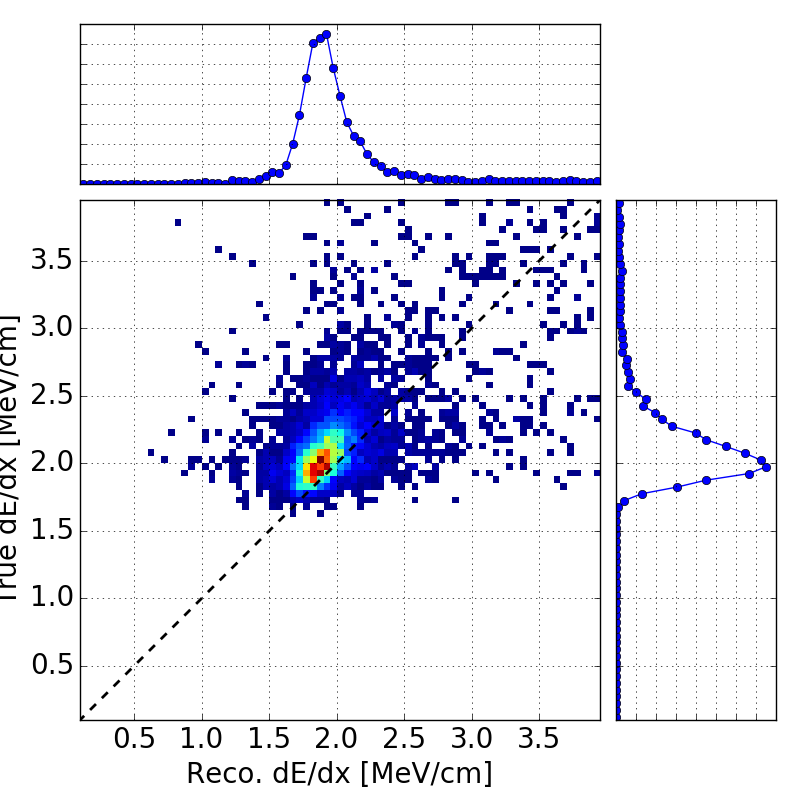
\includegraphics[width=0.45\textwidth]{emshower_figures/e_true_reco_dedx_4cm.png}
  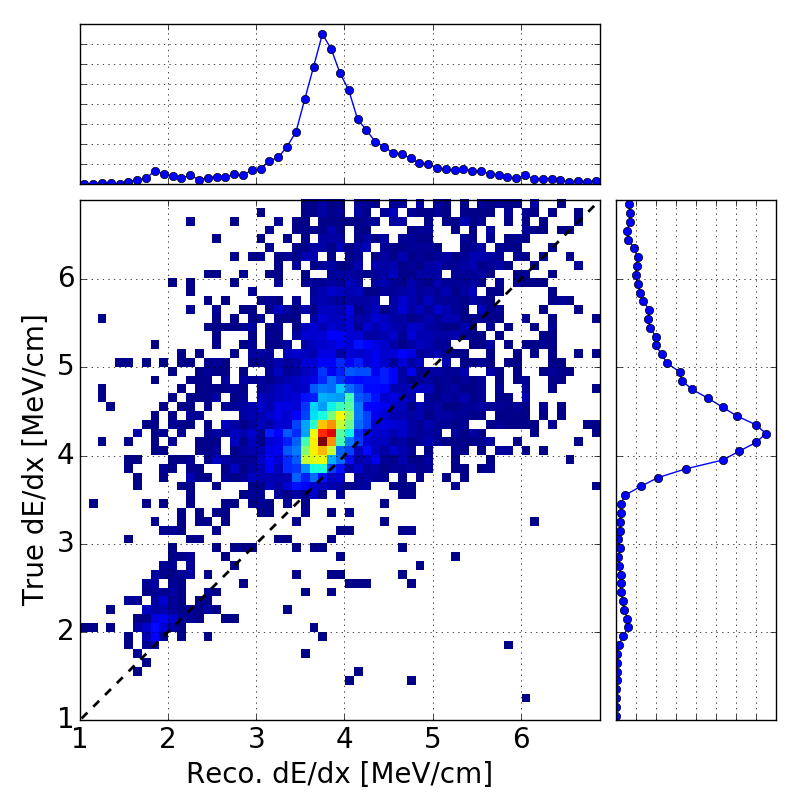
\includegraphics[width=0.45\textwidth]{emshower_figures/p_true_reco_dedx_4cm.png}
  \caption[$dE/dx$ Reconstruction/Monte Carlo Comparision]{The true $dE/dx$ of the beginning of simulated showers, calculated from simulated energy depositions in the TPC, vs the reconstructed $dE/dx$ of the same showers.  The electrons (left) and the gammas (right) both show a strong correlation between true and reconstructed $dE/dx$. There is a small offset arising from reconstruction inefficiencies, below the 10\% level in both electrons and gammas.}
  \label{fig:true_dedx}
\end{figure*}

\FloatBarrier

\section{\label{sec:argo_dedx} Calorimetric Separation of Electromagnetic Showers}

\begin{figure}[htbp]
  \centering
  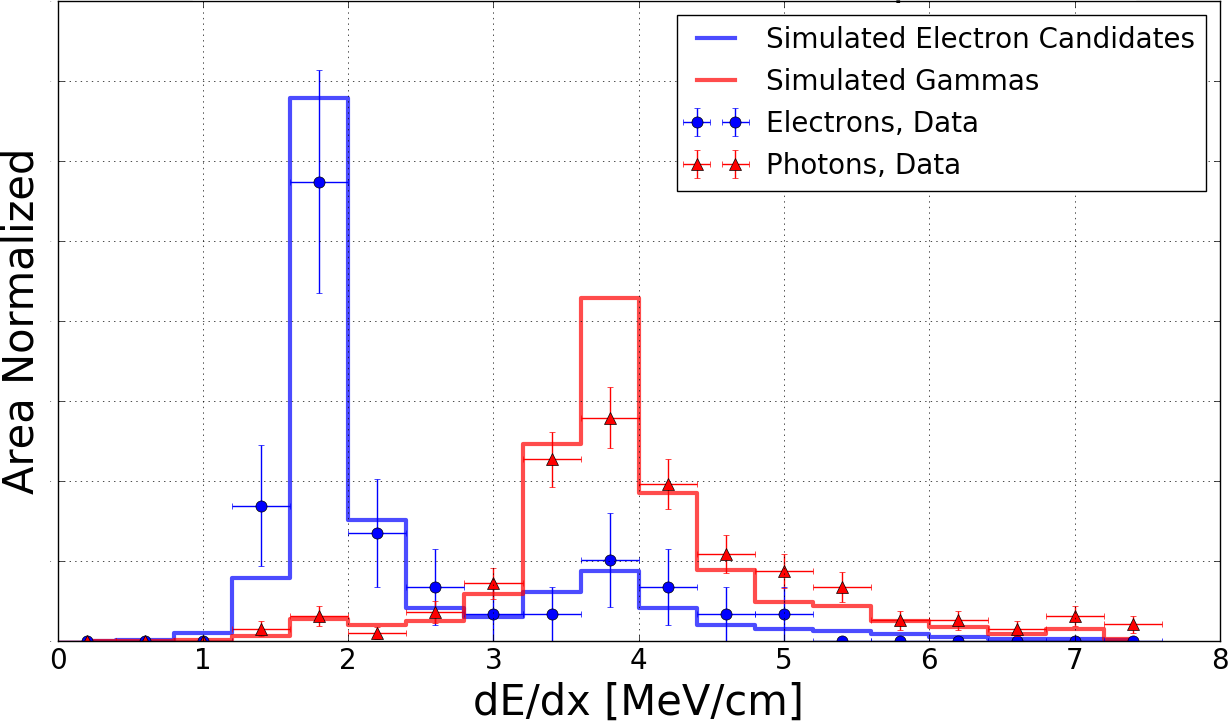
\includegraphics[width=0.99\textwidth]{emshower_figures/median_dedx_trimmed.png}
  \caption[Calorimetric dE/dx Distribution]{The dE/dx distribution for electrons (blue) and gammas (red).  The solid blue curve, representing the simulation of electron dE/dx, includes a 20\% contaimination of gammas consistent with the results from Figure~\ref{fig:electron_landau}.}
  \label{fig:dEdx}
\end{figure}


Figure~\ref{fig:dEdx} represents the first demonstration of calorimetric separation of electrons and gammas in a LArTPC using neutrino events.  Despite the low statistics of the ArgoNeuT experiment, the electron and gamma separation using calorimetry is clearly validated. When a cut is made at 2.9 MeV/cm the efficiency of selecting electron candidate events in data is 76 $\pm$ 7\% with a 7 $\pm$ 2\% contamination from the gamma sample. Here, the uncertainties on the efficiency are estimated with the Feldman-Cousins method \cite{Feldman:1997qc} and are statistical only.  It must be noted, however, that the sample of electron candidates in this figure is not background subtracted.  The efficiency to select electrons with the same cut at 2.9 MeV/cm, estimated with the Monte Carlo, is 91\%.  This is consistent with the above measurement that 20 $\pm$ 15\% of the electron candidate sample, selected by topology only, is in fact gammas.


The value of the cut used above, 2.9 MeV/cm, is also somewhat arbitrary and must be determined uniquely for each analysis.  In this case, it is selected as the mid point between the two peaks of the distribution.  However, in an analysis targeting electron neutrinos the absolute normalization of the electron and gamma shower populations is crucial.  The desired purity of electrons must be balanced with the need to keep sufficient electron statistics.  An aggressive dE/dx cut, at 2.5 MeV/cm, effectively rejects gammas but also can remove a significant amount of electrons (removes 30\% of electron candidate events in data, 13\% of Monte Carlo electrons).  


As seen in figure~\ref{fig:electrons} and figure~\ref{fig:photons}, the high granularity of a LArTPC allows precision topological discrimination of gammas and electrons.  A purely topological cut produced a sample of electron events with an estimated 80 $\pm$ 15\% purity.  Further, full reconstruction of an event can improve gamma rejection.  For example, identification of two electromagnetic showers that reconstruct with an invariant mass consistent with the $\pi^0$ mass can remove both showers as electron candidates, even if there is not a gap present for one shower and the dE/dx cut fails.

The analysis in this chapter has shown, using data, that a metric based on the dE/dx deposition in the beginning part of the shower is a valid method of separating electron-neutrino charged current events from gamma backgrounds. The full gamma background rejection capability of liquid argon detectors will be enhanced by adding to this a topological cut. This represents the first experimental proof of applying the calorimetric cut to separate electrons from gammas in a liquid argon detector using neutrino events.

One should note that the efficiency and misidentification rates presented here do not represent the full capability of liquid argon TPCs to discriminate gamma backgrounds from electron signals. The final separation power of LArTPCs leverages multiple identification techniques, of which calorimetry is just one.  Further, the exact efficiencies and misidentification rates depend heavily on the energy spectrum of the electromagnetic showers: the Compton scattering gammas, a major source of impurity, appear predominately at energies below 200 MeV.


